\newpage
\chapter{Evaluation}

\textbf{Client GUI}

The following features of LoYiW project will be evaluated in this chapter, by running on the network devices, get the following results: 

The following figure shows the result on the browser of mobile device. The first line of the result is MAC - Device - Dict, it display only once,when the program run first time. The target IP on the result means IP address of AP, which is connected to the mobile device. The final line of the result is the MAC address of the AP. The result shows that,the AP has been found, which is connected to the mobile device.

\begin{figure}[!ht]
	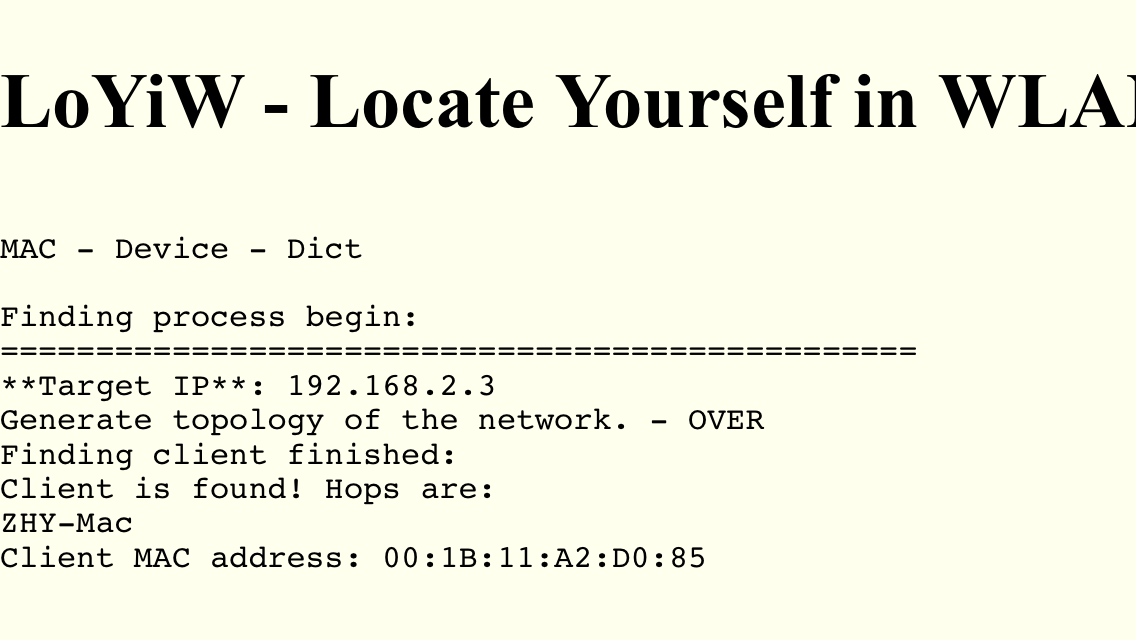
\includegraphics[width=\textwidth]{images/loyiw-run1}
	\caption{Result when the mobile phone is connected to the D-Link}
\end{figure}

The next figure shows that, a device roams from one AP to the next AP,  A new AP information of the target IP and the MAC address is on the result page.

\begin{figure}[!ht]
	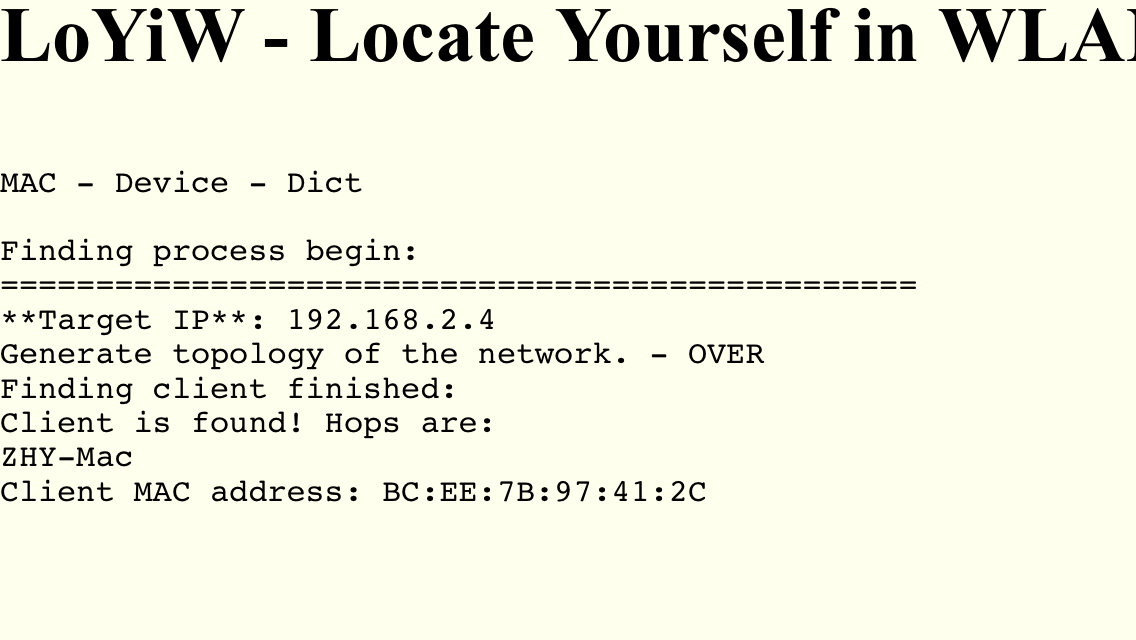
\includegraphics[width=\textwidth]{images/loyiw-run2}
	\caption{Result when the mobile phone is connected to the ASUS RT-N16}
\end{figure}


%\section{Disadvantages of LoYiW}

%Due to differences between the network devices,causing the device can not be found, when the program was running on the devices. 
%\newpage
\textbf{Administration GUI}

The \textit{administration GUI} is programmed by Kivy. Here show the GUI:

\begin{figure}[!ht]
	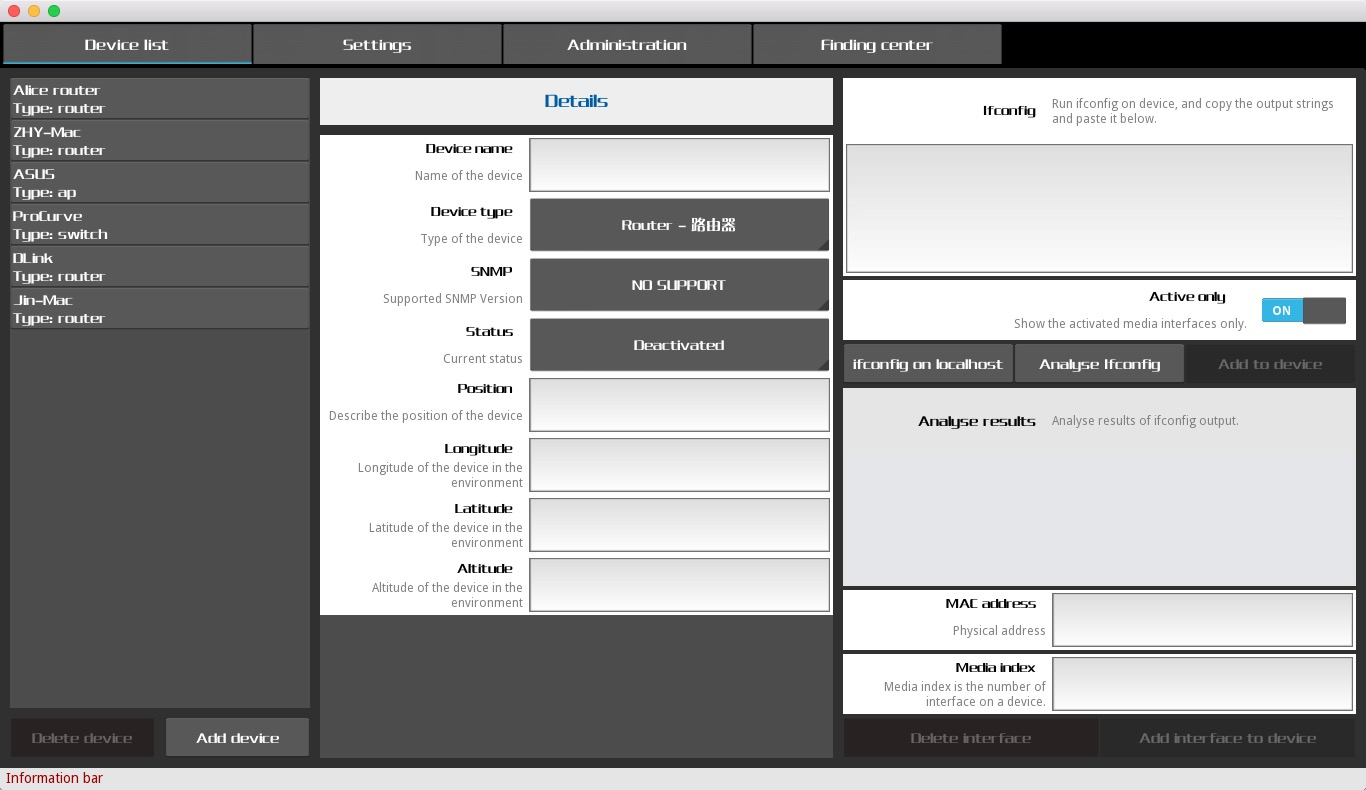
\includegraphics[width=\textwidth]{images/gui1}
	\caption{Devices configuration panel.}
\end{figure}

\begin{figure}[!ht]
	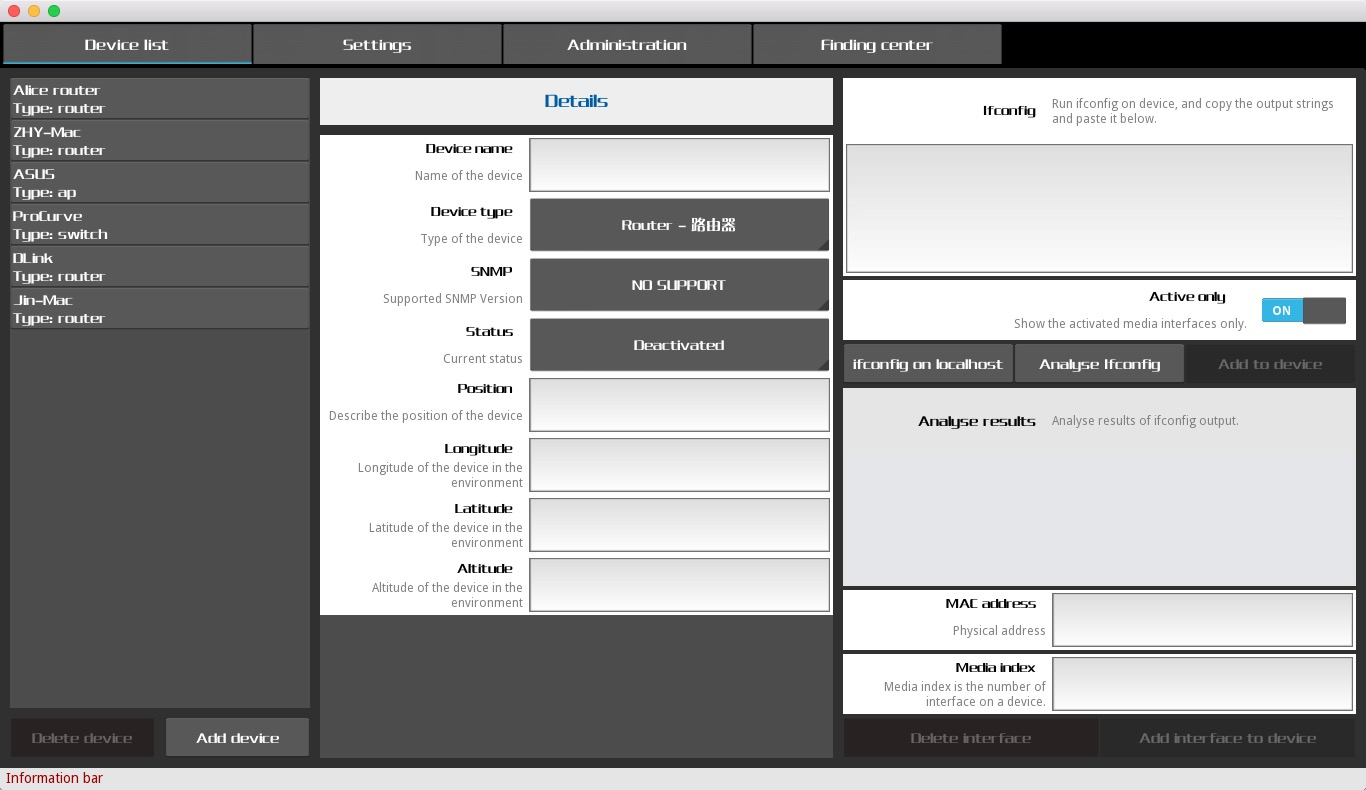
\includegraphics[width=\textwidth]{images/gui1}
	\caption{Settings panel.}
\end{figure}

\begin{figure}[!ht]
	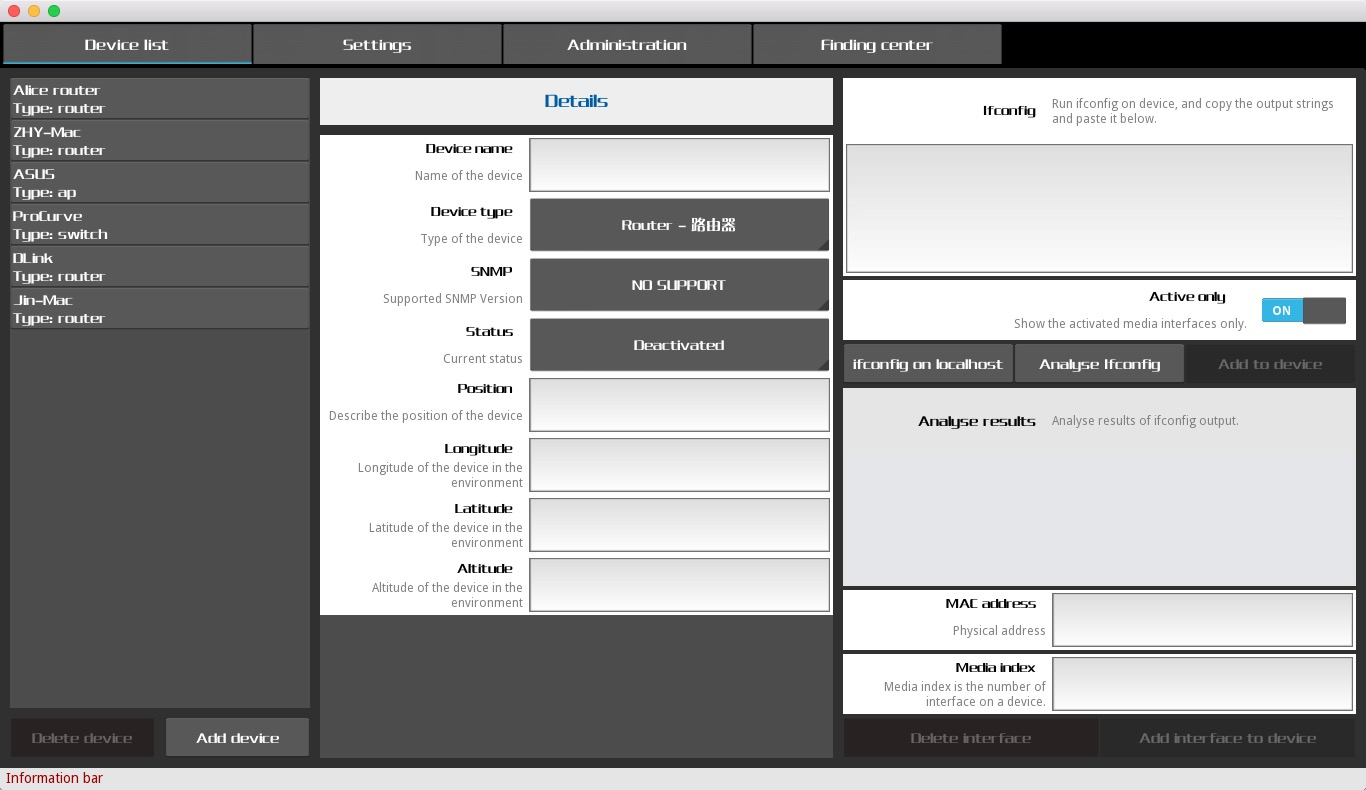
\includegraphics[width=\textwidth]{images/gui1}
	\caption{Control the redirection and server.}
\end{figure}

\begin{figure}[!ht]
	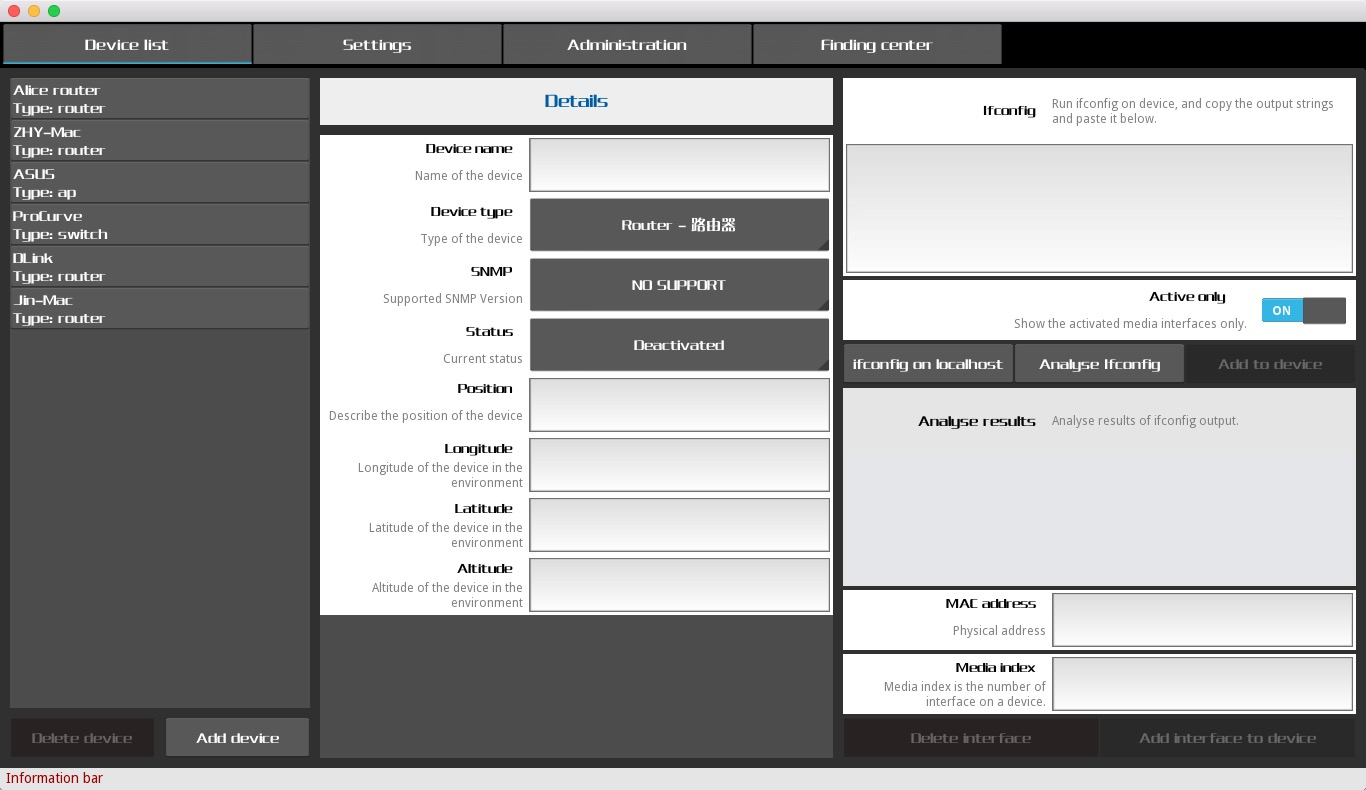
\includegraphics[width=\textwidth]{images/gui1}
	\caption{Find the client device from server side panel.}
\end{figure}
